\documentclass{article}

\usepackage{lastpage} % for the number of the last page in the document
\usepackage{fancyhdr}
\usepackage{geometry}
\usepackage{graphicx}
\usepackage{grffile}
\usepackage[utf8x]{inputenc}
\geometry{a4paper}
\geometry{portrait}
\pagestyle{fancy}
\usepackage{float}
\fancyhf{}
\lhead{User Manual KinderFinder}
\rhead{Section \thesection}
\lfoot{}
\rfoot{Page \thepage\ of \pageref{LastPage}}


%\begin{figure}[H]
%\centering
%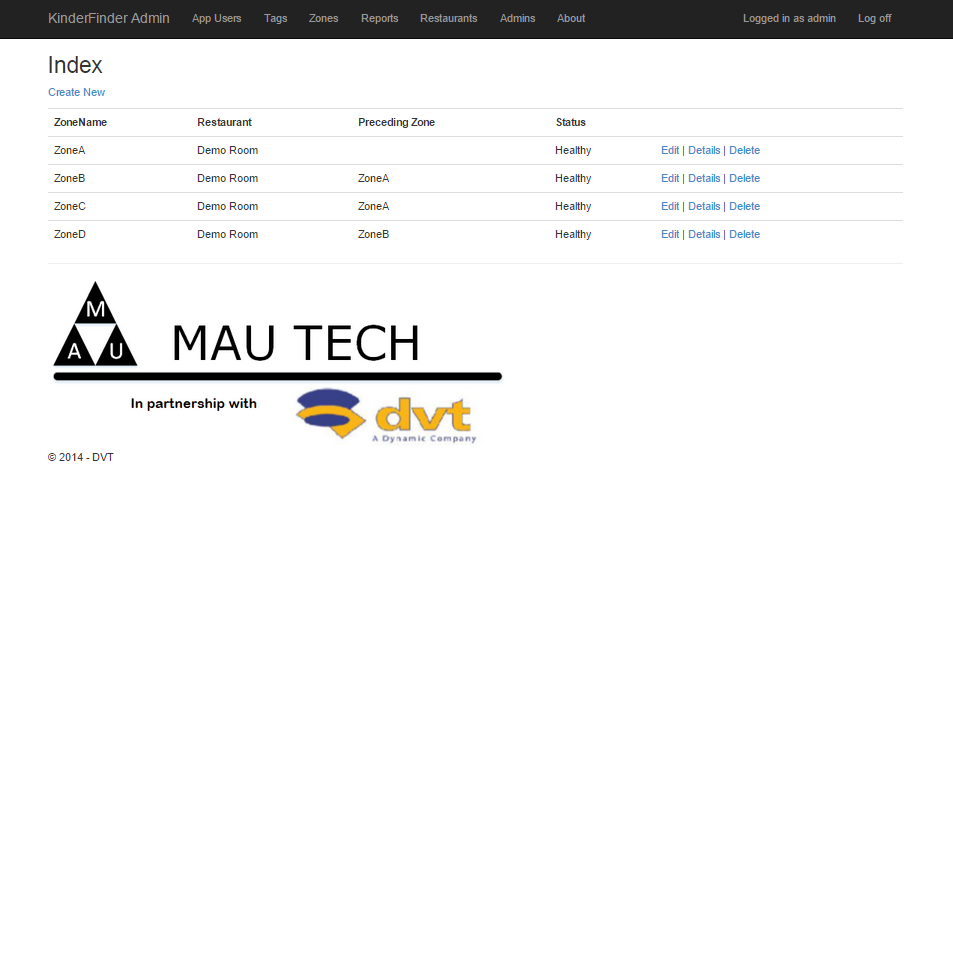
\includegraphics[scale=0.5]{adminportalzones.png}
%\caption{Use case of Android app user (first level granularity).}
%\end{figure}




\begin{document}
\tableofcontents
\newpage


\section{Welcome to KinderFinder}
\subsection{What is KinderFinder}
KinderFinder is a  solution that uses indoor tracking of people ,  to assist with a common 
problem  in  public  places.  Many  restaurants  aim  to  give  parents  a  worry  free  dining 
experience,  by providing facilities to entertain,  and safely look after their children. However, 
a parent still has the worry, and consistent need  to  ensure their children are still in the safe 
and designated areas.  The solution will attempt to assist the parents in being able to make 
sure their children are still in these areas without the need to get up from their tables.


\newpage
\section{About this manual}

\begin{itemize}
\item Please read this manual before using the device to ensure safe and proper use.
\item  	Please read this manual before using the device to ensure safe and proper use.
\item	Descriptions are based on the devices default settings.
\item 	Images and screen shots may differ in appearance from the actual product.
\item 	Content may differ from the final product, or from software provided by service providers 
or carriers, and is subject to change without prior notice.
\item	Content (high quality content) that requires high CPU and RAM usage will affect the 
overall performance of the device. Applications related to the content may not work 
properly depending on the devices specifications and the environment that it is used in.
\item	Available features and additional services may vary by device, software, or service 
provider.

\end{itemize}

\newpage

\section{Getting started}
\subsection{Set up}
Congratulations on your purchase of the KinderFinder system, this manual should help you get the most out if the KinderFinder system installed.

\subsection{Installation}
\subsubsection{Software}
If you are purchasing the KinderFinder software for an establishment, good news, there is minimal installation required.
All software necessary is on the cloud. Navigate on a web browser to www.kinderFinder.co.za to view the Administration Portal that will provide one with the nessessary admin tasks that will be discussed later.

\subsubsection{Room Maps}
As you are aware, KinderFinder uses a map of the room being monitored to view the locations of tags worn by users. In this regard, a map of the room must be made and uploaded to the admin portal. The .JPG format for the map file would be sufficient. On the mobile application it would look similar to figure 1 below.

\begin{figure}[H]
\centering
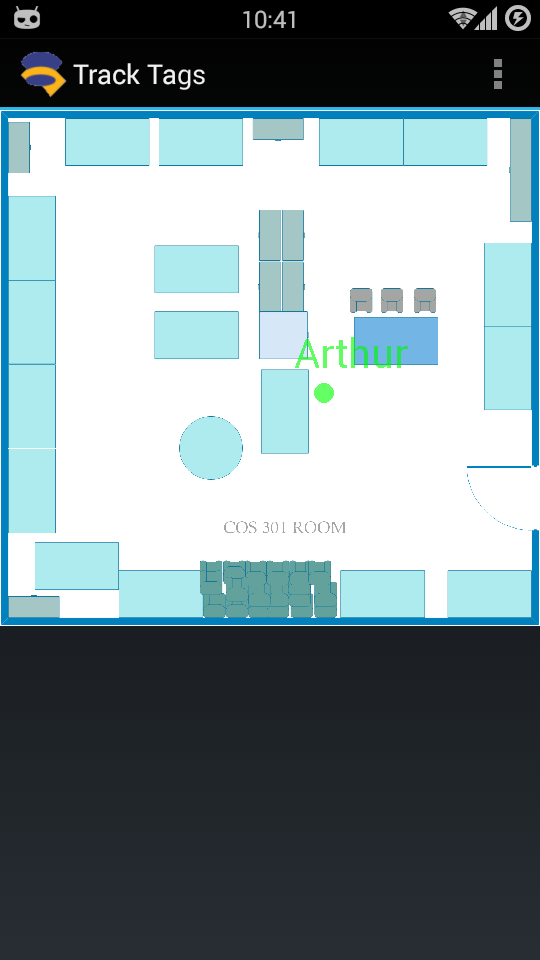
\includegraphics[scale=0.3]{MainAppTrack Tags.png}
\caption{Map view in mobile application}
\end{figure}

\subsubsection{Receivers}
Receivers are devices that pick up the signals from tags worn by users. These receivers should be placed at the edges of the room for maximum range and location capabilities.  Refer to figure 2 for the optimal places to place the receivers.

\begin{figure}[H]
\centering
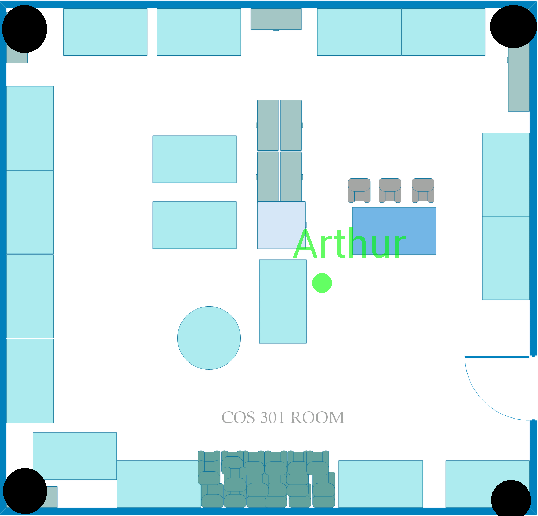
\includegraphics[scale=0.6]{pic1.png}
\caption{Optimal receiver placement}
\end{figure}

\subparagraph{Setting up Receivers}
Receivers used in KinderFinder are android mobile devices. The application that needs to be installed on these devices is called "Transmitter" and should be run from the device. Upon opening the transmitter application, choose the establishment the device will be used in and then the place in the room the device will be in X and Y Cartesian co-ordinates. Tap the "Transmit" button and the application will start to transmit to the server. Do this for all mobile devices used as receivers. 

\end{document}
